% !TEX root = presentation.tex
% { % all template changes are local to this group.
%     \begin{frame}[plain]
%         \begin{tikzpicture}[remember picture,overlay]
%             \node[at=(current page.center)] {
%                 \includegraphics[width=\paperwidth]{./img/03_tomb-raider-underworld}
%             };
%         \end{tikzpicture}
%      \end{frame}
% }


\begin{frame}\frametitle{Properties}
	\begin{quote}
		``Pn triangles should not deviate too much from the original triangle to preserve the shape and avoid interference with other curved triangles.''
		\citeauthor{vlachos2001curved}
	\end{quote}
\end{frame}

\begin{frame}\frametitle{Continuity}
	\todo[inline]{Continuity reference book.}
	PN triangles have:
	\begin{itemize}
		\item $C^1$ continuity in the vertex points
		\item $C^0$ continuity everywhere else
	\end{itemize}
\end{frame}

\begin{frame}\frametitle{Sharp Edges}
	\begin{columns}
		\begin{column}[b]{0.22\textwidth}
			\begin{center}
				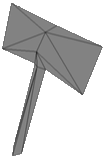
\includegraphics[width=\textwidth]{./img/2_mesh/bluntAxeMesh.png}
				\small{Blunt}
			\end{center}	
		\end{column}
		\begin{column}[b]{0.22\textwidth}
			\begin{center}
				
\includegraphics[width=\textwidth]{./img/2_mesh/bluntAxeShaded.png}
				\small{Blunt}
			\end{center}	
		\end{column}
		\begin{column}[b]{0.22\textwidth}
			\begin{center}
				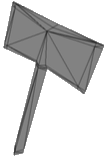
\includegraphics[width=\textwidth]{./img/2_mesh/sharpAxeMesh.png}
				\small{Sharp}
			\end{center}	
		\end{column}
		\begin{column}[b]{0.22\textwidth}
			\begin{center}
				
\includegraphics[width=\textwidth]{./img/2_mesh/sharpAxeShaded.png}
				\small{Sharp}
			\end{center}	
		\end{column}
	\end{columns}
\end{frame}	

\begin{frame}\frametitle{Nvidia}
	\todo[inline]{Nvidia paper}
\end{frame}
